One article~\cite{cpt} introduces the Coherent Path Tracing algorithm (also known
as the CPT algorithm), that is setting a
random seed per sample id within a pixel. It has the hability to increases the
memory cache access by having more parralel rays. But of course that might be
sparsed after severals bounces, cause by material property, or simply because
not intersecting same triangles despites their neighbourhood. Now and GPU, it
would have the same benefit, but not only. Threads in a same warp executed on
GPU cores will share a same compute units(as describe in sub-section~\ref{subsec:warp}). So
if a warp is tracing close and parrellel rays, they would pretty much have
the same memory access pattern, but also the same octree node access. That means
all conditions statement would have an higher probability to be executed (or not)
by all threads. This optimization slices a rendering tile (As described
in \ref{subsec:tile_passes_rendering}) into smaller tiles - that we will call
coherency tiles - having as many pixel sas a warp size have threads. Then we can
actually witness a massive performance improvment on Figure~\ref{table:cpt_compare}.
But as the article~\cite{cpt} says, it generates artefacts as we can see on
Figure~\ref{fig:stanford_bunny_cpt}.

\begin{figure}[h]
    \centering
    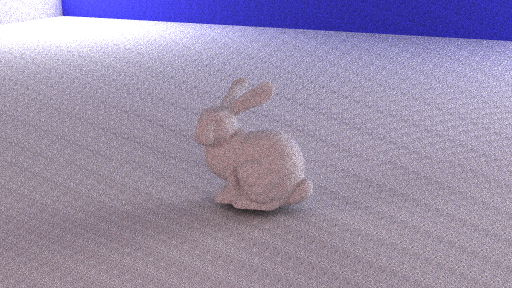
\includegraphics[width=0.8\columnwidth]{render_stanford_bunny_dummy.png}
    \caption{Stanford bunny rendered with a simple path tracer algorithm.}
    \label{fig:stanford_bunny_dummy}
\end{figure}

\begin{figure}[h]
    \centering
    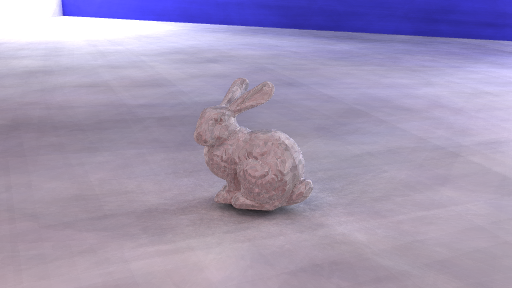
\includegraphics[width=0.8\columnwidth]{render_stanford_bunny_cpt.png}
    \caption{Stanford bunny rendered with a coherent path tracer algorithm.}
    \label{fig:stanford_bunny_cpt}
\end{figure}

\begin{figure}[H]
    \tiny
    \centering
    \begin{tabular}{ | l | c | c | }

        \hline
        Algorithm used & Bunny \\
        \hline
        Simple path tracer & 224.0ns \\
        Coherent path tracer & 101.9ns \\
        \hline

    \end{tabular}
    \caption{
        Per ray rendering time comparaison between a simple path tracer
        algorithm and a coherent path tracer (resolution of 512~x~288; 512
        sample per pixels; 9 recursive raies per samples).
    }
    \label{table:cpt_compare}
\end{figure}
